\chapter{Giới thiệu}
\label{sec:gioithieu}


Chương này nhằm giới thiệu về bài toán sẽ được giải quyết trong luận văn và các khái niệm liên quan. Đầu chương sẽ trình bày về kỹ thuật dịch ngược, các ứng dụng của nó và những khó khăn trong quá trình dịch ngược. Phần tiếp theo nêu bài toán đặt ra và các thách thức khi giải quyết bài toán. Phần cuối cùng sẽ tóm tắt cấu trúc của luận văn.

\section{Kỹ thuật dịch ngược và ứng dụng}
Trong khi kỹ thuật dịch phổ biến hiện nay là dịch từ mã viết bằng ngôn ngữ cấp cao xuống mã ngôn ngữ cấp thấp hơn, kỹ thuật dịch ngược thực hiện dịch từ mã ngôn ngữ cấp thấp lên mã ngôn ngữ cấp cao hơn. Kỹ thuật dịch ngược được sử dụng rất nhiều để hỗ trợ trong quá trình phát triển phần mềm:

\begin{itemize}
	\item Vì một lý do nào đó, mã nguồn của một phần mềm bị mất đi. Để tiếp tục phát triển hoặc bảo trì phần mềm đó, cần phải khôi phục lại mã nguồn. Nếu viết lại một chương trình mới hoàn toàn từ các tài liệu sẵn có sẽ rất mất thời gian và không đảm bảo sẽ tương đương được phần mềm cũ. Vì vậy một giải pháp phổ biến hiện nay là dựa vào file thực thi dịch ngược lại và hiệu chỉnh để có được mã nguồn mới hoàn chỉnh.
	\item Các phần mềm độc hại như virus, malware thường sẽ bị giấu kín mã nguồn. Kỹ thuật dịch ngược giúp sinh ra mã nguồn của chúng, qua đó, việc tìm ra phương pháp giải trừ sẽ dễ dàng hơn.
	\item Một số chương trình được viết để chạy trên các chip đã lỗi thời, như chip 8051, sẽ ngừng sản xuất trong tương lai gần, cần phải được chuyển đổi để chạy được trên những chip hiện đại hơn đang được sản xuất. Một trong những giải pháp để giải quyết vấn đề này là dùng trình dịch ngược để chuyển chương trình viết trên chip lỗi thời sang ngôn ngữ cấp cao, sau đó dùng trình biên dịch để dịch thành mã của chip thay thế. Cấu trúc của hệ thống chuyển đổi này được trình bày ở hình \ref{fig:fig12}.
	
	\begin{figure}[h]
		\centering
		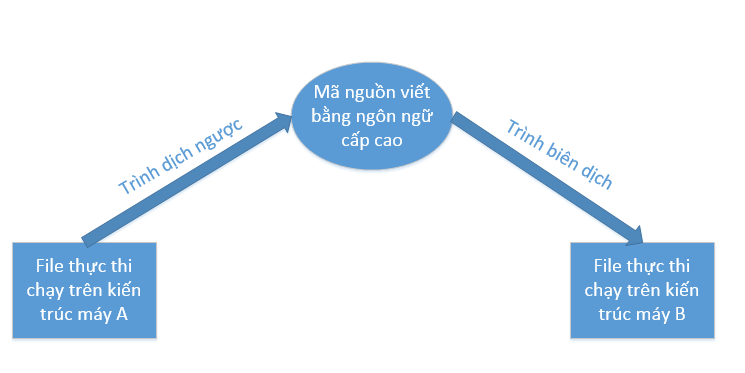
\includegraphics{fig12.png}
		\caption{Một ứng dụng của trình dịch ngược: chuyển đổi mã nguồn giữa các kiến trúc máy khác nhau}
		\label{fig:fig12}
	\end{figure}
	\item Phần mềm viết bằng ngôn ngữ A cần phải chuyển đổi sang ngôn ngữ B để tiếp tục bảo trì và phát triển. Ngôn ngữ A có thể là một ngôn ngữ đã ra đời từ rất lâu (ví dụ: COBOL, Basic...), hiện nay không còn người hiểu biết về ngôn ngữ đó để lập trình phần mềm. Vì vậy, cần phải chuyển đổi phần mềm sang một ngôn ngữ khác mới hơn, có nhân lực để phát triển tiếp (ví dụ: Java, C\#...). Quá trình này cũng được xem là dịch ngược, vì thường ngôn ngữ A ra đời trước sẽ có mức độ trừu tượng thấp hơn là các ngôn ngữ B được phát triển sau này.
\end{itemize}

Một trong những thách thức khó nhất của kỹ thuật dịch ngược là khôi phục thông tin. Do ở các ngôn ngữ cấp thấp không có phương tiện để lưu trữ một số thông tin cần thiết ở ngôn ngữ cấp cao, nên những thông tin đó sẽ bị mất đi trong quá trình dịch xuôi hoặc lập trình bằng ngôn ngữ cấp thấp. Một số thông tin cần khôi phục là:
\begin{itemize}
	\item Kiểu dữ liệu của biến: Đối với các chương trình viết bằng ngôn ngữ cấp cao, kiểu dữ liệu của biến có thể xem như một ràng buộc khi gán giá trị cho biến và sử dụng biến. Ví dụ khi ta khai báo một biến có kiểu dữ liệu là integer, thì ta phải gán cho biến các giá trị là số nguyên (1, 2,...) và sử dụng biến trong các phép toán nhận toán hạng là số nguyên. Nếu ta gán cho biến một giá trị khác số nguyên (số thực, chuỗi, boolean...) hoặc sử dụng biến trong các phép toán không chấp nhận toán hạng là số nguyên thì trình biên dịch sẽ phát hiện lỗi ngay ở giai đoạn đầu. Tuy nhiên, đối với một số mã máy, kiểu dữ liệu không cần thiết và sẽ được loại bỏ trong quá trình biên dịch. Khi dịch ngược, nếu không khôi phục được kiểu dữ liệu thì sẽ không đủ thông tin để xây dựng mã đầu ra.
	
	\item Tên của biến: Ở ngôn ngữ cấp cao, tên biến mang ngữ nghĩa là công dụng của biến đó, và được dùng để truy xuất giá trị của biến. Còn ở ngôn ngữ cấp thấp, dữ liệu sẽ được lưu vào các thanh ghi có sẵn hoặc vùng nhớ được truy xuất bằng địa chỉ trực tiếp, vì vậy việc tên biến ở cấp độ này là không cần thiết và sẽ bị loại bỏ. Nếu trình dịch ngược không giữ được tên biến của chương trình gốc thì rất khó để phát triển và bảo trì. Giải pháp hiện nay của các trình dịch ngược là sinh ra tên biến tự động, sau đó dựa vào các tài liệu sẵn có để chỉnh sửa tên biến bằng tay ở chương trình đầu ra. \cite{ssavan}
	
	\item Phân biệt giữa dữ liệu và mã điều khiển: Đặc điểm của một số mã máy (trừ mã máy chạy trên máy ảo) là dữ liệu và các câu lệnh điều khiển có cùng một định dạng mã nhị phân và được lưu trong cùng một vùng nhớ. Vì vậy, khi dịch ngược từ mã máy lên cần phải phân biệt được phần nào của vùng nhớ là lưu các dữ liệu và phần nào là câu lệnh của chương trình.
\end{itemize}

Từ khái niệm của kỹ thuật dịch ngược, có thể thấy có nhiều mức độ dịch ngược, tương ứng với những bài toán khác nhau cần giải quyết. Dựa vào các ứng dụng, suy ra được đầu vào của một trình dịch ngược có thể là: mã nhị phân, mã assembly hoặc mã của một ngôn ngữ lập trình cấp cao khác cần chuyển đổi. Tùy vào mức độ trừu tượng của ngôn ngữ đầu vào, các thông tin cần khôi phục sẽ khác nhau. Với mã máy thì tất cả các thông tin nêu trên đều không còn. Với mã assembly, tên biến vẫn xuất hiện trong chương trình vì một số assembler cho phép có các câu lệnh khai báo biến ở mã assembly. Còn với mã ngôn ngữ cấp cao thì gần như tất cả thông tin đều có ở chương trình gốc, và vấn đề cần giải quyết là tìm ra các cấu trúc tương đương ở ngôn ngữ đích.

\section{Bài toán đặt ra}
\label{sec:problem}
\subsection{Giới thiệu vấn đề}
Như đã trình bày ở trên, kiểu dữ liệu là một thông tin quan trọng không xuất hiện ở mã cấp thấp nhưng cần phải có để xây dựng mã đầu ra của trình dịch ngược. Vì vậy, bài toán suy luận kiểu là một thách thức cấp bách cần phải giải quyết trong kỹ thuật dịch ngược. Hiện nay, có nhiều nghiên cứu về vấn đề này và đưa ra những giải pháp khác nhau. Tuy nhiên, hầu hết chỉ giải quyết được những kiểu dữ liệu đơn giản như số nguyên, số thực, pointer... Còn các kiểu dữ liệu phức tạp hơn như structure, union, class... vẫn chưa được giải quyết hoàn toàn \cite{ssavan}. Mục tiêu của luận văn là giải quyết vấn đề khôi phục kiểu dữ liệu union. \\

Vấn đề này được đặt ra là do ở một số kiến trúc máy, một đối tượng dữ liệu (thanh ghi hoặc vùng nhớ) có thể được truy xuất ở nhiều cấp độ. Nghĩa là có thể truy xuất toàn bộ đối tượng đó, cũng có thể truy xuất một phần nhỏ hơn của nó. Khi thay đổi một phần đối tượng dữ liệu, thì đồng thời giá trị của toàn bộ đối tượng cũng thay đổi theo và ngược lại, khi thay đổi giá trị đối tượng đó, thì một phần nào đó của nó cũng sẽ thay đổi giá trị. Trong hình \ref{fig:eax}, thanh ghi \textit{eax} có độ dài là \textbf{32 bit}, tuy nhiên, người lập trình có thể truy xuất \textbf{16 bit đầu} của thanh ghi này bằng thanh ghi \textit{ax}. Và tương tự, \textbf{8 bit đầu} và \textbf{8 bit cuối} của \textit{ax} được thể hiện bằng các thanh ghi \textit{ah} và \textit{al}. Như vậy, khi thay đổi giá trị của thanh ghi \textit{ax}, thì giá trị của thanh ghi \textit{eax} cũng sẽ thay đổi theo và ngược lại.\\
\begin{figure}[h]
	\centering
	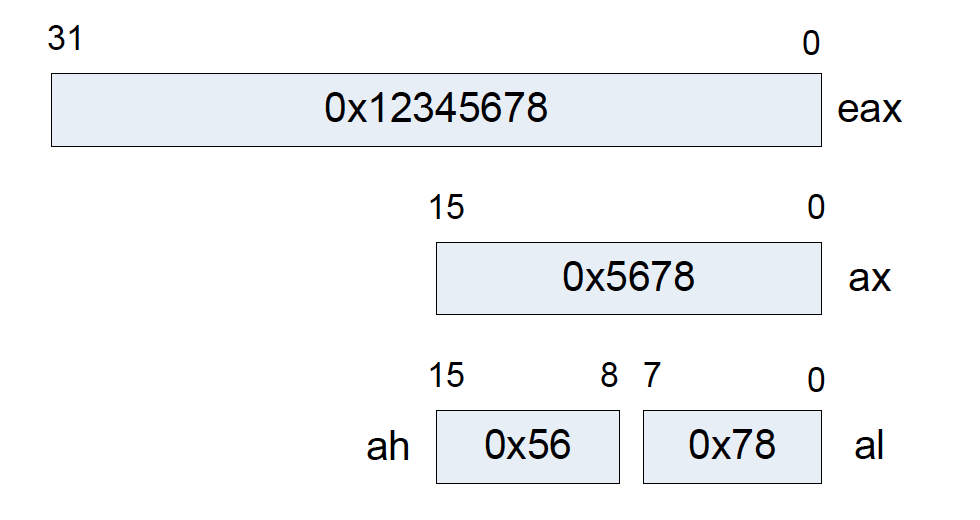
\includegraphics[width=0.7\linewidth]{image/eax}
	\caption{Thanh ghi eax trong kiến trúc máy x86}
	\label{fig:eax}
\end{figure}

Với tính chất trên, không thể xem phần nhỏ hơn của đối tượng dữ liệu (như thanh ghi \textit{ax}, \textit{ah}, \textit{al}) là những biến độc lập ở ngôn ngữ cấp cao, mà phải có cách nào đó thể hiện được mối quan hệ của chúng với toàn bộ đối tượng dữ liệu lớn (như thanh ghi \textit{eax}). Cấu trúc union ở ngôn ngữ cấp cao đáp ứng được yêu cầu đó. Vì cấu trúc union có tính chất là các thành phần cùng chia sẻ một vùng nhớ, nên khi thay đổi giá trị của một thành phần thì các thành phần còn lại cũng thay đổi theo, tương ứng với tính chất nêu trên ở mã assembly của một số kiến trúc máy. Như vậy, ta có thể xem toàn bộ đối tượng dữ liệu là một union với 2 thành phần:
\begin{itemize}
	\item Thành phần 1 cho phép truy xuất đến toàn bộ vùng nhớ.
	\item Thành phần 2 có kiểu dữ liệu là structure, cho phép truy xuất đến những phần nhỏ hơn của vùng nhớ đó.
\end{itemize}

Một trong những kiến trúc máy có những tính chất trên là 8051. Trong 8051, một số thanh ghi có thể được truy xuất ở mức bit, và đồng thời cũng có thể được truy xuất ở mức byte, ví dụ như thanh ghi \textit{ACC}. Như ví dụ trong hình \ref{list:8051exam1}, câu lệnh số 1 gán một giá trị cho thanh ghi \textit{ACC}, trong khi câu lệnh số 2 chỉ sử dụng bit đầu tiên của nó.

\begin{lstlisting}[caption={Đoạn mã 8051 sử dụng thanh ghi ACC ở nhiều cấp độ},label={list:8051exam1}]
MOV A, 38 ;1
SETB ACC.1 ;2
\end{lstlisting}

Ngoài ra, các vùng nhớ của 8051 cũng có tính chất tương tự. Trong ví dụ \ref{list:8051exam}, vùng nhớ có địa chỉ \textbf{38H} được load vào thanh ghi \textit{ACC} thông qua biến \textit{OPTIONS}, và biến \textit{TESTSUPS} đại diện cho bit đầu tiên của \textit{ACC} được sử dụng ngay sau đó. Từ đó, có thể kết luận \textit{ACC} chỉ là công cụ trung gian để thao tác trên vùng nhớ có địa chỉ \textit{OPTIONS} (sau này sẽ gọi tắt là vùng nhớ \textit{OPTIONS}), còn \textit{TESTSUPS} thực chất là bit đầu tiên của vùng nhớ đó. Như vậy, kiểu dữ liệu của vùng nhớ \textit{OPTIONS} là union và \textit{TESTSUPS} là một thành phần của union này.
\begin{lstlisting}[caption={Đoạn mã 8051 có một vùng nhớ mang kiểu union},label={list:8051exam}]
#DEFINE OPTIONS, #38H
#DEFINE TESTSUPS ACC.1
public AA
AA:
MOV A, OPTIONS ;1
SETB TESTSUPS ;2
\end{lstlisting}

\textit{Tóm lại, luận văn sẽ giải quyết vấn đề kiểm tra và suy diễn kiểu union từ mã assembly.} Đối với bài toán kiểm tra kiểu, người lập trình cần phải cung cấp thông tin về các kiểu union được sử dụng thông qua một phương thức nào đó. Chương trình sẽ khai thác thông tin đó và kiểm tra việc sử dụng kiểu union trong mã đầu vào có hợp lý hay không. Còn để suy diễn kiểu union, người lập trình không cần phải cung cấp thông tin, mà trình dịch ngược sẽ tự suy diễn ra các kiểu union thông qua quá trình phân tích việc sử dụng dữ liệu trong chương trình đầu vào. Các giải pháp này được trình bày trong sơ đồ khối \ref{fig:main}.

\begin{figure}
	\centering
	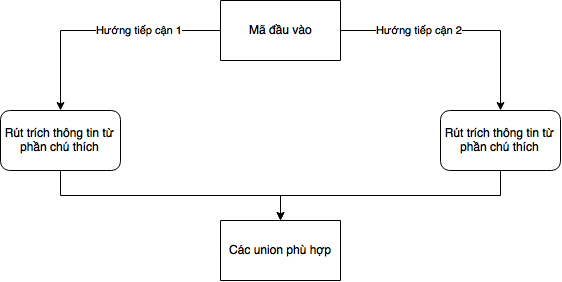
\includegraphics[scale=0.8]{image/main}
	\caption{Cách giải quyết các bài toán được trình bày trong luận văn}
	\label{fig:main}
\end{figure}

\subsection{Giới hạn bài toán}

Trong một kiến trúc máy, có hai kiểu đối tượng được dùng để lưu trữ dữ liệu là thanh ghi và vùng nhớ, luận văn sẽ giải quyết vấn đề khôi phục kiểu union của các vùng nhớ. Đối với các thanh ghi, mỗi kiến trúc máy đã có quy định sẵn thanh ghi nào có thể được truy xuất ở nhiều cấp độ. Một số thanh ghi ví dụ là \textit{eax} trong kiến trúc máy x86 và \textit{ACC} trong kiến trúc máy 8051. Như vậy, chỉ cần đọc đặc tả của kiến trúc máy là có thể biết được các thanh ghi nào có kiểu là union mà không cần phải phân tích gì thêm. Nhưng riêng với vùng nhớ, không có quy định nào đặt ra trước là những vùng nhớ nào được sử dụng như một union, những vùng nhớ nào không được sử dụng như vậy, nên cần trải qua một quá trình phân tích dữ liệu để xác định được kiểu dữ liệu của chúng. Vì vậy, các giải thuật trong luận văn này sẽ tập trung giải quyết vấn đề tìm kiếm kiểu union trên các vùng nhớ.\\

Ngoài ra, có rất nhiều kiến trúc máy có tồn tại kiểu union, nên luận văn sẽ chọn một kiến trúc máy để đưa ra các đoạn mã ví dụ và phân tích, cụ thể đó là 8051. Ngoài việc 8051 có các tính chất phù hợp với yêu cầu, một lý do nữa để chọn kiến trúc máy này là do nó đã lỗi thời và con chip 8051 sẽ bị dừng sản xuất trong tương lai gần, vì vậy, nhu cầu chuyển đổi mã từ 8051 sang một kiến trúc máy khác hiện đại hơn là có thật. Việc xây dựng giải thuật trên 8051 sẽ có thể ứng dụng ngay vào trình dịch ngược cho hệ thống chuyển đổi đó, giúp đưa ra kết quả chính xác hơn. Tuy nhiên, các giải thuật được nêu ra trong luận văn hoàn toàn có thể được áp dụng với những kiến trúc máy khác có tính chất tương tự 8051.

\subsection{Thách thức của bài toán}

Thách thức khó khăn nhất của bài toán là việc xác định các thành phần của một union đại diện cho vùng nhớ vì các thông tin ban đầu không đủ để kết luận điều đó. Như trong ví dụ \ref{list:8051exam}, thông tin ở phần khai báo ban đầu chỉ cho biết \textit{OPTIONS} mang giá trị là \textbf{38H}, và \textit{TESTSUPS} đại diện cho bit đầu tiên của thanh ghi \textit{ACC}, không có cơ sở nào để kết luận \textit{TESTSUPS} là một thành phần của union đại diện cho vùng nhớ \textit{OPTIONS}. Phải trải qua một quá trình phân tích dữ liệu, chỉ ra được rằng mỗi khi chương trình thao tác trên \textit{TESTSUPS}, thanh ghi \textit{ACC} luôn được load vào dữ liệu của vùng nhớ \textit{OPTIONS}, hay nói cách khác là thanh ghi ACC mang kiểu union \textit{OPTIONS}, thì mới xác định được \textit{TESTSUPS} là một thành phần thuộc union \textit{OPTIONS}. Như vậy, mấu chốt của bài toán là phải tìm ra được kiểu dữ liệu mà thanh ghi đóng vai trò trung gian đang mang và đây là một vấn đề phức tạp, đòi hỏi phải nghiên cứu nhiều phương pháp phân tích khác nhau để đưa ra được phương pháp có độ chính xác cao nhất và có thời gian xử lý chấp nhận được.


\section{Cấu trúc luận văn}

Luận văn gồm có 6 chương. Chương tiếp theo sẽ trình bày về các kiến thức nền tảng, cũng như một số nghiên cứu liên quan đến kỹ thuật dịch ngược. Ngoài ra, chương này cũng chỉ rõ kiến trúc của trình dịch ngược Boomerang và phần mở rộng của nó, nền tảng được dùng để hiện thực các nghiên cứu của luận văn. Chương 3 nêu ra giải pháp cho bài toán Kiểm tra kiểu. Tiếp theo đó, chương 4 trình bày cách giải quyết bài toán tiếp theo là Suy luận kiểu. Chương 5 giới thiệu một số thiết lập cần thiết trên trình dịch ngược Boomerang để kiểm tra kết quả các giải pháp đã đề ra ở những chương, cách thiết lập các mẫu thử (testcase) và kết quả chạy thử. Chương 6 kết luận về kết quả đạt được của luận văn và đề ra các hướng nghiên cứu tiếp theo.
	
\begin{comment}
Như đã đề cập ở phần trên, mục tiêu của luận văn là nghiên cứu về trình dịch ngược từ mã assembly lên mã cấp cao, các bài toán cần phải giải quyết và hiện thực giải pháp. Vì mã assembly cho kiến trúc máy khác nhau có những đặc điểm khác nhau, và đi cùng với đó là những vấn đề khác nhau cần giải quyết, nên giới hạn của luận văn sẽ là trình dịch ngược từ mã assembly 8051. Việc chọn kiến trúc máy 8051 là do 2 nguyên nhân sau:
\begin{itemize}
	\item Chip 8051 đã xuất hiện trên thị trường từ lâu, hiện tại sắp không còn được sản xuất. Tuy nhiên, vẫn còn nhiều hệ thống được chạy trên đây và cần phải chuyển đổi chúng sang một kiến trúc máy khác hiện đại hơn. Như vậy, nhu cầu đặt ra là có thực.
	\item Chip 8051 có một số đặc điểm khác biệt so với các con chip khác trên thị trường. Vì vậy việc dịch ngược từ mã 8051 sẽ gặp nhiều khó khăn hơn, vấn đề phải giải quyết phức tạp hơn. 
\end{itemize}

Các đặc điểm khác biệt của 8051 gồm có:
\begin{itemize}
	\item Trong khi hầu hết các kiến trúc máy khác sử dụng kiểu dữ liệu byte là kiểu dữ liệu nhỏ nhất, thì 8051 cho phép lập trình viên truy xuất tới mức bit trong một số thanh ghi và kèm theo đó là các câu lệnh xử lý bit. Tuy nhiên, các thanh ghi này của 8051 cũng có thể được truy xuất ở mức byte bình thường. Xem ví dụ ở đoạn mã \ref{list:list1}, câu lệnh số 1 gán giá trị ở vùng nhớ có địa chỉ 38H cho toàn bộ thanh ghi ACC, trong khi câu lệnh số 2 chỉ sử dụng biến số 1 của thanh ghi ACC.
	\begin{lstlisting}[caption={Một đoạn mã 8051 sử dụng cả biến bit và biến byte của thanh ghi ACC},label={list:list1}]
	MOV ACC, 38H #1
	SETB ACC.1 #2
	\end{lstlisting}
	\item Một số assembler của 8051 cho phép sử dụng tên biến. Biến này dùng để lưu các giá trị hằng số, hằng số này thường là địa chỉ một vùng nhớ kích thước 1 byte (trong luận văn này sẽ gọi tắt là biến byte) hoặc đại diện cho bit của thanh ghi (gọi tắt là biến bit). Khi lập trình, người ta thường sử dụng biến byte và biến bit này theo bộ, nghĩa là chỉ khi thanh ghi được load vào giá trị vùng nhớ quy định bởi biến byte, thì các biến bit cùng bộ mới được sử dụng (xem ví dụ ở đoạn mã \ref{list:list2}) (từ nay, khi luận văn sử dụng từ "nguyên tắc sử dụng bộ biến", nghĩa là đang đề cập đến nguyên tắc này).
		\begin{lstlisting}[caption={Một đoạn mã 8051 tuân theo nguyên tắc sử dụng bộ biến},label={list:list2}]
	#DEFINE OPTIONS #38H
	#DEFINE TESTSUP ACC.1
	public AA
	AA: 
	MOV ACC, OPTIONS
	JB TESTSUP, BB
	\end{lstlisting}
\end{itemize}

Từ các đặc điểm trên, ta có thể thấy bài toán lớn nhất đặt ra trong luận văn này sẽ là tìm ra được mối liên hệ giữa biến byte và biến bit trong chương trình, lấy được các bộ biến byte và biến bit đúng. Có 2 cách để biết được điều này:
\begin{itemize}
	\item Đưa ra quy định về việc khai báo biến byte và biến bit. Hiện nay, ở phần khai báo, các lập trình viên có thể khai báo các biến theo thứ tự tuỳ ý, và cũng không có quy định nào bắt buộc họ phải có phần comment chỉ rõ các biến byte và biến bit nào là cùng một bộ. Ta có thể đưa ra các mẫu khai báo cho biến byte và biến bit để trình dịch ngược có thể biết được các bộ biến bằng cách đọc theo mẫu mà không cần phân tích gì thêm. Tuy nhiên, sau khi đã xác định được các bộ biến này, cần có thêm một bước kiểm tra mã chương trình để đảm bảo rằng nguyên tắc sử dụng biến byte và biến bit được tuân thủ. Vì vậy, ta sẽ gọi giải pháp này là Kiểm tra kiểu - Type checking. Giải pháp này có ưu điểm là đơn giản, dễ hiện thực nhưng gây bất tiện cho người dùng vì phải chuyển đổi bộ mã hiện tại về theo mẫu quy định.
	\item Dựa vào phân tích luồng dữ liệu của chương trình, tìm ra được địa chỉ vùng nhớ được load vào thanh ghi tại thời điểm sử dụng biến bit và từ đó suy ra biến byte cùng bộ với biến bit đó. Giải pháp này được đặt tên là Suy luận kiểu - Type inference. Với cách làm này, không cần phải thay đổi đoạn mã gốc. Tuy nhiên cách hiện thực sẽ phức tạp hơn nhiều vì có rất nhiều cách load dữ liệu vùng nhớ vào thanh ghi như: dùng trực tiếp hằng số, dùng trực tiếp biến byte, trung gian qua một thanh ghi khác, dùng một biểu thức toán học có 2 vế... (xem ví dụ ở đoạn mã \ref{list:list3})
		\begin{lstlisting}[caption={Ví dụ một số mẫu câu lệnh load vùng nhớ vào thanh ghi trong 8051},label={list:list1}]
	MOV ACC, 38H
	MOV ACC, OPTIONS
	MOV ACC, @DPTR
	MOV ACC, OPTIONS+1
	\end{lstlisting}
\end{itemize}

Cả hai giải pháp này đều được hiện thực trong từng giai đoạn của luận văn và sẽ được trình bày trong các chương tiếp theo.

Ngoài ra, một công việc khác cần phải làm đó là giữ nguyên tên biến trong quá trình dịch ngược. Hiện tại trình dịch ngược Boomerang chỉ cho phép ta định nghĩa trước một số thanh ghi trong một kiến trúc máy, và đoạn mã đầu vào chỉ được sử dụng các thanh ghi đó, nếu sử dụng một cái tên nằm ngoài danh sách thanh ghi thì sẽ báo lỗi. Vì vậy, ta sẽ phải điều chỉnh cơ chế này, cho phép việc sử dụng tên biến khác và giữ nguyên chúng khi dịch ra đoạn mã ngôn ngữ cấp cao.

\section{Cấu trúc luận văn}
Luận văn sẽ gồm 6 chương như sau:
\begin{itemize}
	\item Chương 1: Giới thiệu về kỹ thuật dịch ngược, bài toán đặt ra trong luận văn và cấu trúc của luận văn.
	\item Chương 2: Nêu lên một số kiến thức cơ bản và các nghiên cứu liên quan đến luận văn. Đặc biệt, trong chương này sẽ trình bày một số kiến thức cơ bản về Boomerang, giúp người đọc dễ dàng hiểu các phần sau hơn.
	\item Chương 3: Trình bày giải pháp Kiểm tra kiểu - Type checking. Ngoài ra, trong chương này sẽ trình bày cơ chế cho phép đọc tên biến khác thanh ghi và lưu trữ chúng trong trình dịch ngược, vì đây là bước đầu tiên trong quá trình thực hiện các giải pháp.
	\item Chương 4: Trình bày giải pháp Suy luận kiểu - Type inference.
	\item Chương 5: Đánh giá kết quả của luận văn thông qua các mẫu thử (testcase).
	\item Chương 6: Kết luận.
\end{itemize}
\end{comment}